\section{Requests}
\label{sec:requests}

The goal of this assignment is to write an elastic-plastic stress update algorithm for simple shear deformation using MATLAB.
It is important to note that this algorithm is independent of the finite element analysis and is strictly on the implementation of computational plasticity.
This implementation is similar to writing a custom user-defined material subroutine (UMAT) for commercial FE software, with the exception that you must obtain the kinematic variables across time.

\begin{figure}[h]
    \centering
    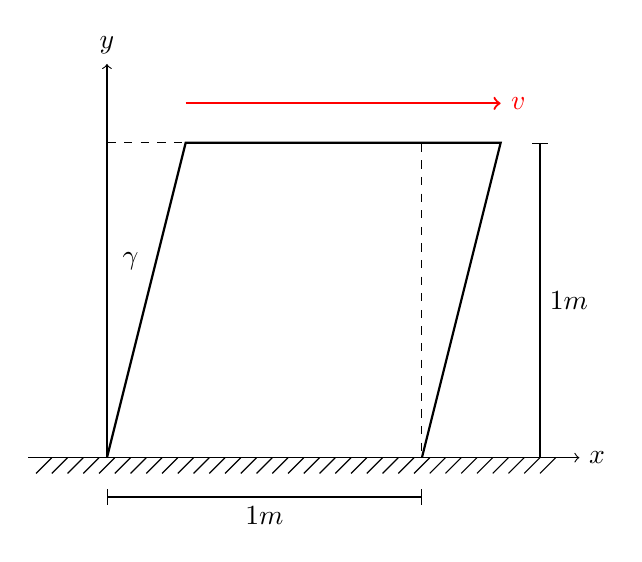
\begin{tikzpicture}

        \draw[->] (-1, 0) -- ++(7, 0) node[right]{$x$};
        \draw[->] (0, 0) -- ++(0, 5) node[above]{$y$};

        \draw[thick] (0, 0) -- ++(1, 4) -- ++(4, 0) -- ++(-1, -4);
        % \draw[thick] (2, 0) -- ++(1, 4);
        % \draw[thick] (0.5, 2) -- ++(4, 0);

        \draw[dashed] (0, 0) -- ++(0, 4) -- ++(4, 0) -- ++(-0, -4);
        % \draw[dashed] (2, 0) -- ++(0, 4);
        % \draw[dashed] (0, 2) -- ++(4, 0);

        \draw[|-|] (0, -0.5) -- ++(4, 0) node[midway, below]{$1m$};
        \draw[|-|] (5.5, 0) -- ++(0, 4) node[midway, right]{$1m$};

        \draw[->, thick, red] (1, 4.5) -- ++(4, 0) node[right]{$v$};

        \node at (0.3, 2.5) {$\gamma$};

        \foreach \x in {-0.7, -0.5, ..., 5.7}
        \draw (\x, 0) -- ++(-0.2, -0.2);

    \end{tikzpicture}
    \caption{Problem representation in its initial (dashed lines) and final (solid lines) configuration.}
    \label{fig:problem_representation}
\end{figure}

Consider a square-shape aluminum plate under simple shear deformation.
The deformation gradient for simple shear is:

\begin{equation}
    F = \begin{bmatrix}
        1 & \gamma \\
        0 & 1
    \end{bmatrix}
\end{equation}

\begin{itemize}
    \item Obtain infinitesimal strain in the simple shear problem when the shear deformation is linearly increased from zero to $\gamma = 1$. Use constant time increments.
    \item Implement von-Mises plasticity according to the radial return algorithm described in the lecture notes. Use the following elastic constitutive equation in modeling of the elastic-plastic deformation. Do not consider kinematic hardening.
\end{itemize}

\begin{equation}
    \dot{\sigma} = C : \dot{\varepsilon}
\end{equation}

Plot the shear stress as a function of shear strain, $\gamma$.

Assume the material has a Young's modulus $E = 70 \text{GPa}$ and a Poisson's ratio of $\nu = 0.3$.
During plastic deformation, the material hardens according to the following isotropic hardening equation

\begin{equation}
    \bar{\sigma} = \sigma_{Y0} + K (\bar{\varepsilon}^p)^n
\end{equation}

where $\sigma_{Y0} = 200 \text{MPa}$, $K = 325 \text{MPa}$, and $n = 0.125$.

\begin{itemize}
    \item Use the following elastic constitutive equation instead of the one at the second request and compare the
    results
\end{itemize}

\begin{equation}
    \sigma^{oT} = C : D
\end{equation}

Is there any significant difference between the results? Why?

$\sigma^{oT}$ is the Truesdell rate of Cauchy stress and $D$ is the rate-of-deformation tensor.

% \begin{table}[H]
%     \centering
%     \begin{tabular}{|c|c|c|}
%         \hline
%         \textbf{Parameter} & \textbf{Value} & \textbf{Unit}                    \\ \hline
%         $E$                & $70$           & $\text{GPa}$                     \\ \hline
%         $\nu$              & $0.3$          & $\text{-}$                       \\ \hline
%         $\rho$             & $2700$         & $\text{kg/m\textsuperscript{3}}$ \\ \hline
%         $L_x$              & $1$            & $\text{m}$                       \\ \hline
%         $L_y$              & $1$            & $\text{m}$                       \\ \hline
%     \end{tabular}
%     \caption{Parameters of the plate element.}
%     \label{tab:parameters_of_the_system}
% \end{table}
